\documentclass[11pt]{article}

\usepackage[utf8]{inputenc}
\usepackage{tabularx}
\usepackage{hyperref}
\usepackage{array}  
\usepackage{graphicx} % Per inserire immagini (loghi)
\usepackage{geometry} % Per personalizzare i margini
\usepackage{fancyhdr} % Per gestire intestazioni e piè di pagina
\usepackage{tikz}
\usepackage{ragged2e}
\usepackage{anyfontsize}
\usepackage[table,xcdraw]{xcolor}
\usepackage{tabularx, etoolbox} % aggiungi etoolbox per condizioni% Load xcolor
\usepackage{eso-pic} % Per aggiungere elementi grafici su tutte le pagine

\graphicspath{{images/}}

\setcounter{secnumdepth}{4}


%cambio misure della pagina
\geometry{a4paper,left=25mm,right=25mm,top=25mm,bottom=25mm}
%ebdfc7
\definecolor{colorePie}{HTML}{ebdfc7}
\pagestyle{fancy}
\fancyhf{}
\renewcommand{\headrulewidth}{0.4pt}
\lhead{
    \parbox[c]{1cm}{
\includegraphics[width=1.1cm]{Sevenbitslogo.png}}
}
\rhead{\textcolor[HTML]{9e978a}{ ANALISI DEI REQUISITI v0.2.0}
}
\setlength{\headheight}{25pt}
\cfoot{\thepage}




\renewcommand*\contentsname{Indice}
\renewcommand{\listfigurename}{Elenco delle figure}

\begin{document}

% Pagina del titolo
\begin{titlepage}
    \setcounter{page}{0}
    \centering
    % Inserisci il logo del gruppo (modifica il percorso dell'immagine)
    
\includegraphics[width=7.2cm]{Sevenbitslogo.png} \\[2cm] 
    
    % Titolo
     {\fontsize{40}{40}\bfseries Analisi dei Requisiti}\selectfont \\[3.9em]
    
    % Sottotitolo
    {\huge NearYou\\ \vspace{3mm }Smart custom advertising platform} \\[2.7em]
    
    % Email del gruppo
    {\large sevenbits.swe.unipd@gmail.com} \\[3em]
    
    % Spazio per il logo dell'università
    \hfill
    
        
    \AddToShipoutPictureBG{ % Imposta il triangolo con logo
        \ifnum\value{page}=0
        \begin{tikzpicture}[overlay]
        
            % Definisce un triangolo blu in basso a destra
            \fill[colorePie] 
                (current page.south east) -- ++(-9cm,0) -- ++(9cm,9cm);
            
            % Inserisce il logo all'interno del triangolo
            \node[anchor=south east, xshift=-0.3cm, yshift=0.3cm] at (current page.south east) {
                
\includegraphics[width=4.5cm]{LogoUnipd.png}
            };
        \end{tikzpicture}
        \fi
    }
        
    

    \vfill % Aggiunge spazio verticale per centrare il contenuto
\end{titlepage}
\newpage
\clearpage
\setcounter{page}{1}



\centering\textbf{Registro modifiche}\\
\vspace{2mm}
\begin{tabular}{|l|l|l|l|l|l|}
\hline
\textbf{Versione} & \textbf{Data} & \textbf{Autore} & \textbf{Verificatore} & \textbf{Descrizione} \\
\hline
0.2.0 & 2024-11-21 & Uncas Peruzzi  & Federico Pivetta & Migliorie varie e inizio\\
& & & & redazione sez.3 (Casi d'uso) \\
\hline
0.1.1 & 2024-11-15 & Uncas Peruzzi  & Riccardo Piva & Redazione sez.1 e sez.2 \\
\hline
0.1.0 & 2024-11-14 & Uncas Peruzzi  & Riccardo Piva & Inizio redazione del documento\\
\hline
\end{tabular}
\newpage
\tableofcontents
\listoffigures %elenco delle figure sarà da usare per ogni immagine
%degli use cases , utilizzando begin figures, caption ecc..

\newpage
\begin{justify}
    

\section{Introduzione}


\subsection{Scopo del documento}

Il seguente documento ha l'obiettivo di fornire una descrizione accurata dei casi d'uso e dei requisiti riguardanti il progetto \textit{"NearYou - 
Smart custom advertising platform"} concernenti al Capitolato C4 proposto da \href{https://www.synclab.it/home}{SyncLab} e aggiudicato al gruppo dal committente.


\subsection{Glossario}
Con l'intendo di evitare ambiguità interpretative del linguaggio utilizzato, viene fornito un Glossario che si occupa di esplicitare il significato dei termini che riguardano il contesto del progetto. I termini presenti nel glossario sono contrasegnati con una \textit{G} a pedice : Termine\(_G\).\\
Le definizioni sono presenti nell'apposito documento \textit{Glossario v1.0.0}


\subsection{Riferimenti}


\subsubsection{Riferimenti normativi}
\begin{itemize}
    \item[-] ISO/IEC/IEEE 29148:2018(E) \\
    \textcolor{blue}{\texttt{\url{https://ieeexplore.ieee.org/stamp/stamp.jsp?tp=&arnumber=8559686}}}
    
    \item[-] Regolamento del progetto didattico  \\
    \textcolor{blue}{\texttt{\url{https://www.math.unipd.it/~tullio/IS-1/2024/Dispense/PD1.pdf}}}
    
\end{itemize}
\subsubsection{Riferimenti informativi}
\begin{itemize}
    \item[-] Capitolato C4- NearYou - 
Smart custom advertising platform\\
    \textcolor{blue}{\texttt{\url{https://www.math.unipd.it/~tullio/IS-1/2024/Progetto/C4p.pdf}}}
    \item[-] Analisi dei Requisiti - SWE 2024-25\\
    \textcolor{blue}{\texttt{\url{https://www.math.unipd.it/~tullio/IS-1/2024/Dispense/T05.pdf}}}
    \item[-] Analisi e descrizione delle funzionalità: Use Case e relativi diagammi (UML) - SWE 2024-25\\    
    \textcolor{blue}{\texttt{\url{https://www.math.unipd.it/~rcardin/swea/2022/Diagrammi\%20Use\%20Case.pdf}}}
    \item[-] Verbali Interni
    \item[-] Verbali Esterni
    
\end{itemize}

\newpage
\section{Descrizione del prodotto}
\subsection{Obiettivi del prodotto}

Il prodotto software da sviluppare, ha il principale obiettivo di generare annunci personalizzati per l'utente, sulla base della sua profilazione e posizione in tempo reale sulla mappa, tramite l'utilizzo dei LLM , nel momento in cui si trovi su un veicolo (dotato di display). Il risultato desiderato, prevede di proporre agli utenti esclusivamente annunci finalizzati a catturare il loro interesse, con il fine di massimizzare il tasso di engagement.
\subsection{Ambito del prodotto}
Il campo di applicazione del prodotto software \textit{NearYou - 
Smart custom advertising platform}, è focalizzato per clienti che offrono un servizio di renting di mezzi di trasporto, dotati di display, nei quali durante l'itinerario di viaggio vengano presentate pubblicità mirate in base a:
\begin{itemize}
    \item [-] sensori di posizione (GPS);
    \item [-] informazioni date dagli utenti in fase di iscrizione;
    \item [-] informazioni di stato fisico dell’utente.
\end{itemize}

\subsection{Panoramica del prodotto}
\subsubsection{Prospettiva generale del prodotto} 
In questa sezione vengono elencate tutte le interfacce di sistema che possono interagire con il prodotto \textit{Near You}.

\paragraph{Interfacce utente}\mbox{}\\
\textit{Near You} è un prodotto che offre un interfaccia utilizzabile su display touchscreen ,con la quale l'utente può interagire visivamente e fisicamente. Nell'ambiente di sviluppo del prodotto, il display è emulato tramite una web-app che presenta una mappa interattiva, sulla quale vengono visualizzate pubblicità associate ai punti di interesse. Per l'utente privilegiato,che offre il servizio di renting, è presente dashboard nella quale è possibile visualizzare la mappa, con tutte le posizioni live dei mezzi e i vari punti di interesse, se generati dal software sottostante.
\paragraph{Interfacce hardware}\mbox{}\\
Il prodotto sviluppato sfrutta i dati monitorati e acquisiti da sensori, nel contesto di sviluppo saranno dati generati attraverso simulazioni reali. Il display touchscreen, corrisponderà a una web-app accessibile da un web browser. Come risultato di quanto detto lo sviluppo del progetto non avviene con elementi hardware fisici.

\subsubsection{Funzionalità del prodotto}
Il prodotto software dovrà garantire le seguenti caratteristiche:
\begin{itemize}
    \item [-] permettere all'utente di creare un profilo dettagliato in modo da poter raccogliere dati significativi.
    \item [-] la simulazione dati provenienti dai sensori GPS, nel caso del percorso effettuato dall'utente, deve corrispondere a coordinate di itinerari che esistono realmente.
    \item [-] separazione del flusso di dati generato dai simulatori, tramite l'utilizzo di un broker opportuno, facilitando di fatto la gestione delle informazioni tra i diversi componenti del sistema.
    \item [-] individuazione dei punti di interessi specifici, sfruttando LLM, che prende in input i dati di profilazione e posizione.
    \item [-] serializzazione dei dati precedentemente menzionati, in un database adatto e performante alla tipizzazione degli input.
    \item [-] acquisizione e processazione dei dati dei sensori,per mezzo di uno strumento adatto allo stream processing,per fornirli in pasto al framework di generative AI.
    \item [-] fornire un'interfaccia di visualizzazione dati, sia lato utente che cliente, per il primo sono richiesti percorso e visualizzazione degli annunci personalizzati, per il secondo una dashboard interattiva.
    
\end{itemize}

\subsubsection{Caratteristiche degli utenti}
Gli utenti si possono distinguere in utente privilegiato, il quale offre il servizio di renting del mezzo e il noleggiatore designato come un normale utente.\\
L'utente privilegiato, deve poter accedere a una dashboard per visualizzare il tracking gps dei vari mezzi di trasporto, e gli ultimi punti di interesse generati per essi.
L'utente tipico di \textit{Near You} è un individuo a bordo di un veicolo, dotato di display, che fornisce , durante il tragitto eventuali annunci personalizzati affini a punti di interesse generati ad hoc.
\subsubsection{Limitazioni}
Non è stata segnalata da parte del proponente, alcuna limitazione o problematica relativa alla privacy nella raccolta dati dell'utente e nella fase di sviluppo del prodotto.
\\
Sono invece note nel documento \textit{Piano di Progetto v1.0.0} restrizioni, che riguardano il tempo a disposizione e il budget allocato per lo sviluppo del progetto. 
\newpage
\section{Casi d'uso}
\subsection{Finalità e specifiche}
Questa sezione espone una serie di casi d'uso, come risultato di un'analisi dei requisiti continuativa del capitolato, dal confronto con la proponente e dalle riflessioni degli Analisiti del team. La specifica di ogni caso d'uso segue gli standard descritti in maniera dettagliata nel documento Norme di Progetto v1.0.0.

\subsection{Attori}
Di seguito sono elencati gli attori con i quali si intefaccia il sistema:
\begin{itemize}
    \item \textbf{Utente privilegiato}: nel nostro dominio di sviluppo coincide con il nolleggiatore dei mezzi di trasporto, che deve poter accedere alla dashboard con il tracciamento dei propri mezzi, previa autenticazione ???
    \item \textbf{Utente}: è il soggetto utilizzatore del servizio di renting, che visualizza la mappa con gli eventuali punti di interesse.
    \item \textbf{Sensore}: è un dispositivo che raccoglie dati di posizione geografica, che sono letti e utilizzati del sistema.
\end{itemize}
\subsection{Elenco dei casi d'uso}
%modello da seguire copia incolla
% \subsubsection{\textbf{UC1.0 - Visualizzazione Dashboard}}
% \begin{itemize}
%     \item \textbf{Attore Principale:}
%     \item \textbf{Precondizioni:}
%     \item \textbf{Postcondizioni:}
%     \item \textbf{Scenario Principale:}
%     \item \textbf{User story associata:}
%     \item \textbf{Estensioni:}
% \end{itemize}
\subsubsection{\textbf{UC1.0 - Visualizzazione Dashboard}}
\begin{itemize}
    \item \textbf{Attore Principale:} Utente privilegiato.
    \item \textbf{Precondizioni:} Il sistema è operativo e accessibile.
    \item \textbf{Postcondizioni:} l'utente privilegiato è in grado di visualizzare una mappa geografica, con i sensori GPS aggiornati in tempo reale (marker) e le varie pubblicità offerte agli utenti.
    \item \textbf{Scenario Principale:}
    \begin{enumerate}
        \item L'utente privilegiato accede alla piattaforma di visualizzazione della dashboard.
        \item Il sistema mette a disposizioni tutte le informazioni storicizzate e ricevute dai sensori, distribuiti su una mappa tramite marker.
    \end{enumerate}
    \item \textbf{User story associata:} Come utente privilegiato, voglio accedere alla dashboard per visualizzare in tempo reale i mezzi che ho messo a noleggio (sensori GPS) e le inserzioni che vengono generate.
    
\end{itemize}
\begin{figure}[ht]
    \centering
    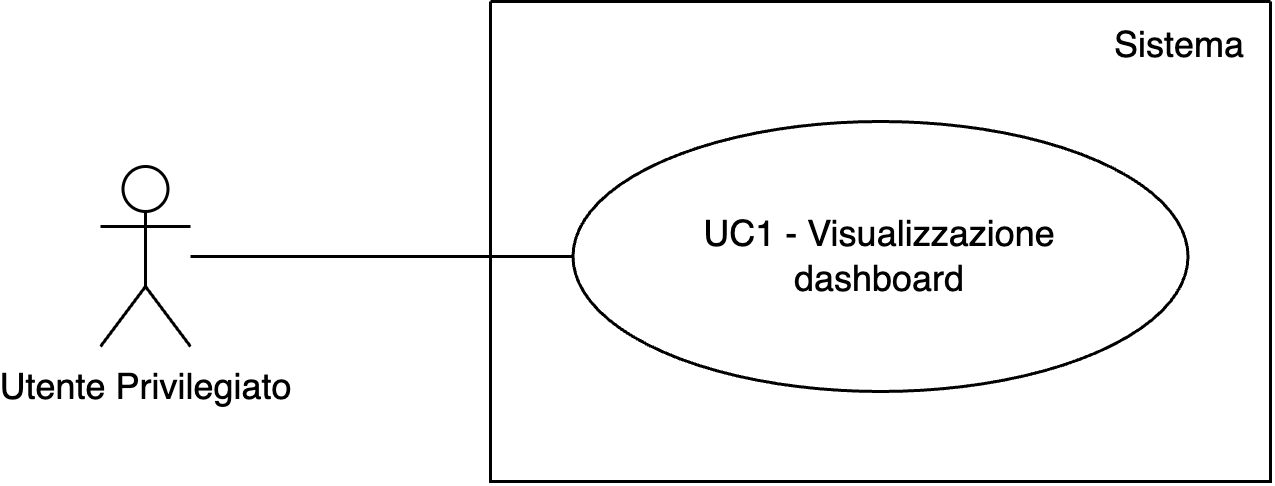
\includegraphics[width=0.5\linewidth]{UC1image.png}
    \caption{UC1 - Visualizzazione Dashboard}
    \label{fig:UC1}
\end{figure}

\subsubsection{\textbf{UC1.1 - Visualizzazioine dettagli dei marker sulla mappa }}
\begin{itemize}
     \item \textbf{Attore Principale:} Utente Privilegiato.
     \item \textbf{Precondizioni:} Il sistema è operativo e accessibile.
     \item \textbf{Postcondizioni:} l'utente privilegiato è in grado di ottenere informazioni più dettagliate dell'utente selezionando il marker visibile sulla mappa.
     \item \textbf{Scenario Principale:}
     \begin{itemize}
         \item L'utente privilegiato ha accesso alla dashboard con la mappa interattiva (UC1).
         \item L'utente privilegiato seleaziona un marker per vederne informazioni più dettagliate.
         \item Il sistema mette a disposizione il dato più recententemente archiviato per quel marker.
     \end{itemize}
     \item \textbf{User story associata:}
     Come utente privilegiato voglio selezionare i vari marker , che indicano i mezzi di trasporto, presenti sulla mappa , in modo da vedere i dettagli sulla posizione e sull'utente che sta utilizzando il mezzo.
\end{itemize}
\begin{figure}[ht]
    \centering
    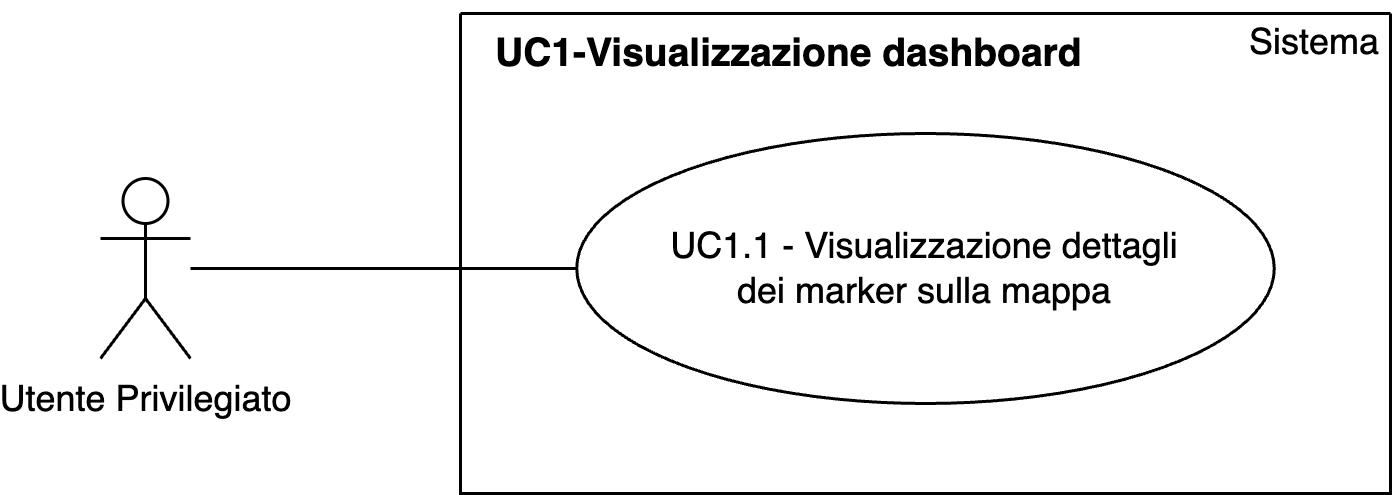
\includegraphics[width=0.5\linewidth]{UC1.1image.png}
    \caption{UC1.1 - Visualizzazioine dettagli dei marker sulla mappa}
    \label{fig:UC1.1}
\end{figure}



\newpage
\section{Requisiti}
%sicuramente da suddividere intenamente tra obbligatori, desiderabilli e opzionali
\subsection{Requisiti funzionali}
\subsection{Requisiti di usabilità}
\subsection{Requisiti prestazionali}
\subsection{Requisiti di vincolo}


\end{justify}
\end{document}
